\appendix

\section{Beispiele}

\begin{figure}[h!]\centering
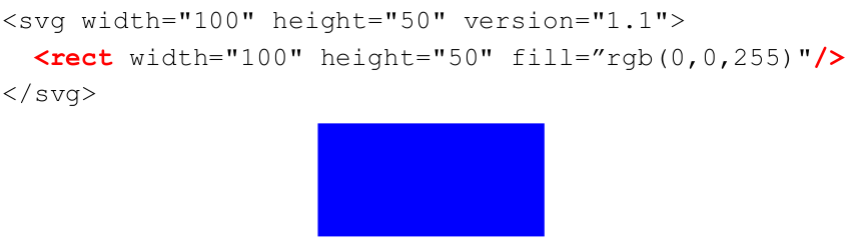
\includegraphics[width=0.6\textwidth]{pictures/rect.png}
\caption{Ein Viereck blau ausgefüllt.}
\label{fig:rect}\end{figure}
\begin{figure}[h!]\centering
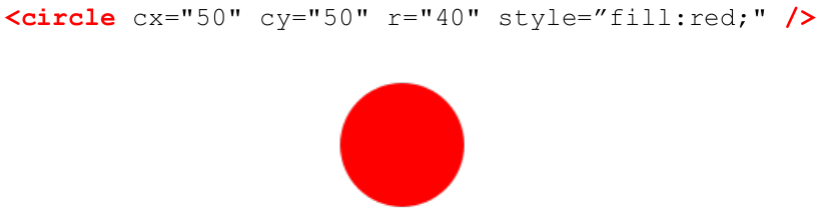
\includegraphics[width=0.6\textwidth]{pictures/circle.png}
\caption{Ein Kreis rot ausgefüllt.}
\label{fig:circle}\end{figure}
\begin{figure}[h!]\centering
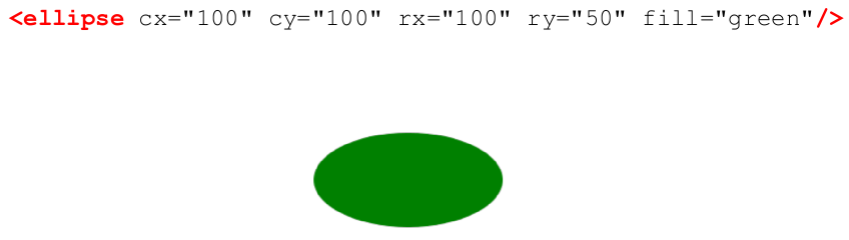
\includegraphics[width=0.6\textwidth]{pictures/ellipse.png}
\caption{Eine Ellipse grün ausgefüllt.}
\label{fig:ellipse}\end{figure}
\begin{figure}[h!]\centering
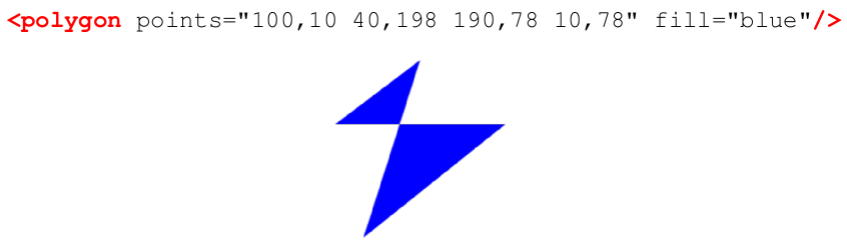
\includegraphics[width=0.6\textwidth]{pictures/polygon.png}
\caption{Beispielhaftes Polygon mit vier Punkten.}
\label{fig:poly}\end{figure}
\begin{figure}[h!]\centering
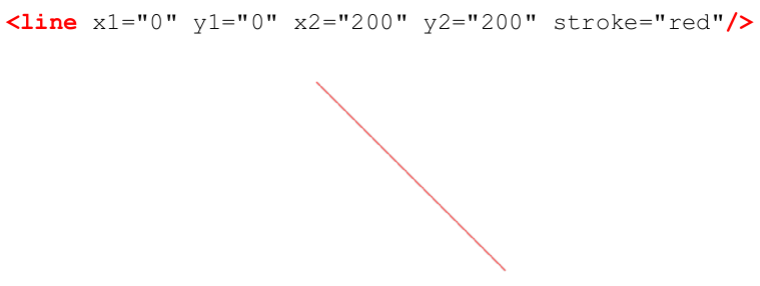
\includegraphics[width=0.6\textwidth]{pictures/line.png}
\caption{Eine einfache Linie.}
\label{fig:line}\end{figure}
\begin{figure}[h!]\centering
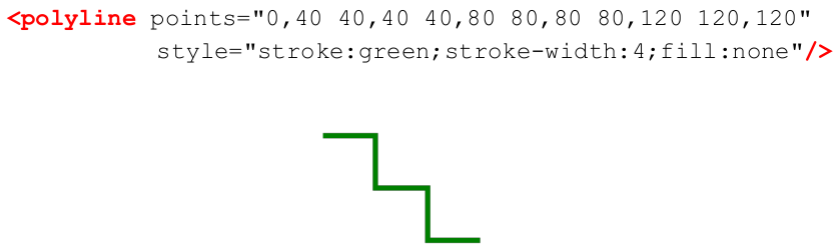
\includegraphics[width=0.6\textwidth]{pictures/polyline.png}
\caption{Einfache Polyline mit sechs Punkten.}
\label{fig:polyl}\end{figure}
\begin{figure}[h!]\centering
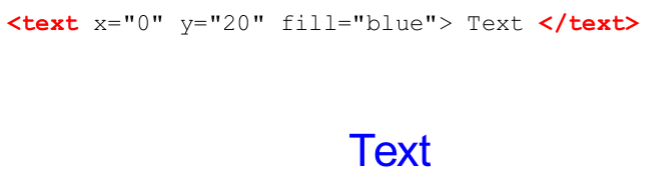
\includegraphics[width=0.6\textwidth]{pictures/text.png}
\caption{Ein einfacher Text in SVG.}
\label{fig:text}\end{figure}
\begin{figure}[h!]\centering
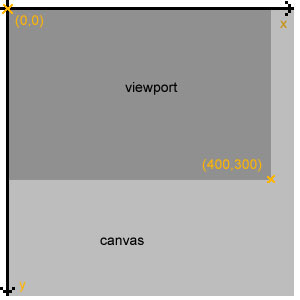
\includegraphics[width=0.3\textwidth]{pictures/koordinatensystem.jpg}
\caption{Koordinatensystem mit Canvas und Viewport.}
\label{fig:koor}\end{figure}
\begin{figure}[h!]\centering
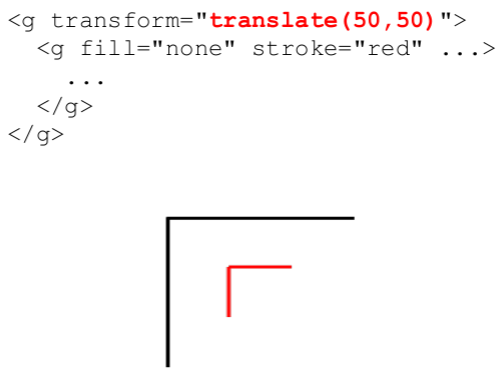
\includegraphics[width=0.6\textwidth]{pictures/transla.png}
\caption{Translation des ursprünglichen Koordinatensystems (schwarz) um jeweils 50 in x- und y-Richtung.}
\label{fig:trans}\end{figure}
\begin{figure}[h!]\centering
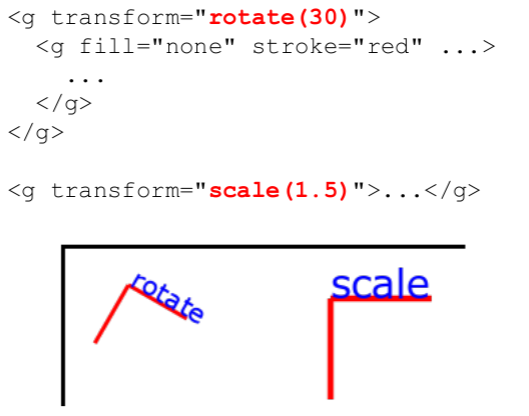
\includegraphics[width=0.6\textwidth]{pictures/rot_scal.png}
\caption{Links eine Rotation um 30. Rechts eine Vergrößerung um 1.5.}
\label{fig:rot}\end{figure}
\begin{figure}[h!]\centering
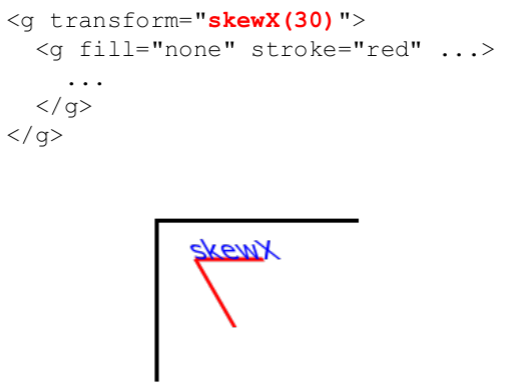
\includegraphics[width=0.6\textwidth]{pictures/skew.png}
\caption{Verzerrung um 30.}
\label{fig:skew}\end{figure}
\begin{figure}[h!]\centering
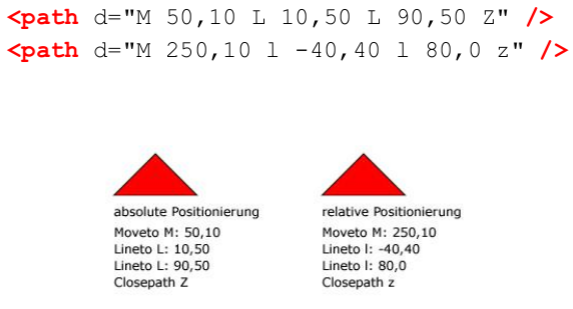
\includegraphics[width=0.6\textwidth]{pictures/path.png}
\caption{Links Pfad mit absoluter Positionierung. Rechts das gleiche Objekt mit relativer Positionierung.}
\label{fig:path}\end{figure}
\begin{figure}[h!]\centering
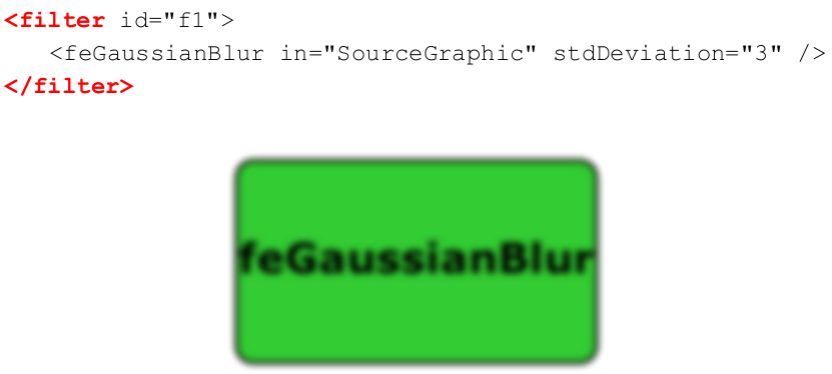
\includegraphics[width=0.6\textwidth]{pictures/filter.png}
\caption{Beispielhafter gaußscher Filter.}
\label{fig:filter}\end{figure}
\begin{figure}[h!]\centering
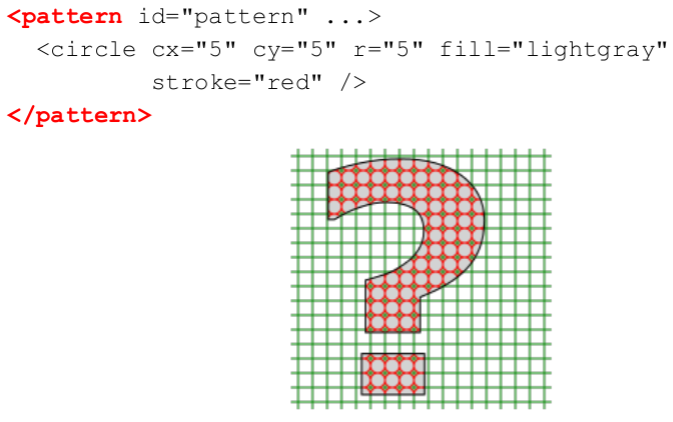
\includegraphics[width=0.6\textwidth]{pictures/pattern.png}
\caption{Das Fragezeichen wurde mit selbst definiertem Muster ausgefüllt.}
\label{fig:pattern}\end{figure}
\begin{figure}[h!]\centering
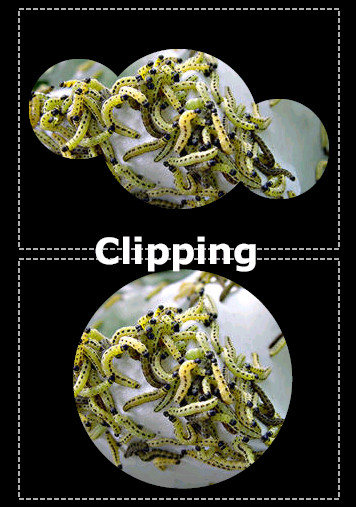
\includegraphics[width=0.3\textwidth]{pictures/kap14_1.jpg}
\caption{Beispielhaftes Clipping eines Bildes.}
\label{fig:clip}\end{figure}

\newpage